\documentclass[sigconf]{webmedia}

% \usepackage{lmodern}  % removido: o próprio template proíbe lmodern (substitui a Libertine e quebra a matemática)
%webmeda.cls is adapted from acmart.cls for use in Proceedings of the Brazilian Symposium on Multimedia and the Web (WebMedia)
\usepackage[brazilian]{babel}
\usepackage{multirow}
\graphicspath{{../results/figures/}}

%%
%% \BibTeX command to typeset the BibTeX logo in the docs
\AtBeginDocument{%
  \providecommand\BibTeX{{%
    \normalfont B\kern-0.5em{\scshape i\kern-0.25em b}\kern-0.8em\TeX}}}

\settopmatter{printacmref=false, printfolios=false}

%% Choose the appropriate event.
\setevent{webmedia}
\proceedingsDetails[WebMedia’2026]{Proceedings of the Brazilian Symposium on Multimedia and the Web}{2026}{Lavras/MG, Brazil}
\ISSN{2966-2753}

\newcommand{\repo}{\url{https://github.com/danielbcsantana/tp-grafos}}

%% end of the preamble, the start of the body of the document source.
\begin{document}

\title[Análise da Rede P2P Gnutella (p2p-Gnutella06)]{Análise Estrutural e Algorítmica da Rede P2P Gnutella (p2p-Gnutella06)}
\subtitle{Trabalho Prático --- Teoria dos Grafos (MATA53), UFBA}

\author{Daniel Santana}
\email{danielbcsantana10@gmail.com}
\affiliation{%
  \institution{Instituto de Computação, Universidade Federal da Bahia}
  \city{Salvador}
  \state{BA}
  \country{Brasil}}

\renewcommand{\shortauthors}{Santana}

\begin{abstract}
Este trabalho analisa o grafo \textit{p2p-Gnutella06} do repositório SNAP, uma
captura da rede \textit{peer-to-peer} Gnutella feita em 6 de agosto de 2002
(8.717 vértices e 31.525 arestas). Após o tratamento dos dados (conversão para grafo
simples não direcionado, que já é conexo), calculamos as métricas estruturais
exatas. Implementamos BFS, DFS, verificação de eulerianidade, Dijkstra,
Bellman-Ford, Floyd-Warshall, Tarjan, Prim e Kruskal, e comparamos a complexidade
teórica com o tempo real medido (30 execuções, IC de 95\%). Por fim, avaliamos a
propriedade de mundo pequeno, a hipótese de lei de potência e a robustez a falhas e
ataques. O grafo tem caminhos curtos ($L=4{,}57$, diâmetro 10) e clusterização
8,2 vezes maior que a de um grafo aleatório equivalente, o que indica um mundo
pequeno fraco. A distribuição de graus é bimodal e não segue lei de potência.
A rede é robusta a falhas aleatórias e moderadamente sensível a ataques aos
vértices de maior grau. A principal descoberta é que a forma do grafo é dominada
pelo processo de coleta: 57\% dos vértices nunca foram rastreados, e não existe
nenhuma aresta entre dois deles.
\end{abstract}

\keywords{teoria dos grafos, redes complexas, SNAP, Gnutella, mundo pequeno, lei de potência, robustez}

\maketitle

\section{Introdução}
O objetivo deste trabalho é aplicar os conceitos da disciplina a um grafo real. O
trabalho cobre o tratamento dos dados, a análise estrutural, a implementação dos
algoritmos clássicos com análise de complexidade e a interpretação de propriedades
de redes complexas (mundo pequeno, lei de potência e robustez). Todo o código, os
dados tratados e as instruções de execução estão no repositório \repo.

\section{Determinação do grafo}
Para a matrícula $M = 224216274$, a soma dos dígitos é
$2+2+4+2+1+6+2+7+4 = 30$ e os dois últimos dígitos são $74$. Assim,
\[
f(M) = \big(30 \times (74+1)\big) \bmod 129 = 2250 \bmod 129 = 57,
\]
pois $2250 = 17 \times 129 + 57$. O índice 57 da planilha
\textsc{Analisando-SNAP-Dataset} corresponde ao grafo \textbf{G57 = p2p-Gnutella06}
(categoria \textit{Internet peer-to-peer networks}).

\section{Descrição do grafo original}
O \textit{p2p-Gnutella06} faz parte da coleção SNAP~\cite{snapnets}. É uma de nove
capturas da rede Gnutella feitas em agosto de 2002~\cite{leskovec2007,ripeanu2002}.
Os vértices são \textit{hosts} da rede e as arestas são conexões entre eles. O
arquivo descreve um grafo \textbf{dirigido} com 8.717 vértices e 31.525 arestas, sem
pesos, sem atributos e sem informação temporal. O cabeçalho do arquivo informa que
cada par não ordenado de vértices é gravado uma única vez.

\section{Tratamento realizado}\label{sec:tratamento}
Os tratamentos foram feitos em \texttt{src/01\_tratamento.py}:
\begin{enumerate}
  \item remoção das linhas de comentário do arquivo SNAP;
  \item verificação de auto-laços e de arestas repetidas: \textbf{nenhum} foi encontrado;
  \item \textbf{dirigido $\rightarrow$ não direcionado}: cada arco $u\rightarrow v$
  vira a aresta $\{u,v\}$. Como não há pares recíprocos ($u\rightarrow v$ e
  $v\rightarrow u$), nenhuma aresta foi fundida e o grafo simples resultante tem
  31.525 arestas. Usamos a versão não direcionada porque conexões P2P são
  bidirecionais (as mensagens trafegam nos dois sentidos);
  \item \textbf{extração da maior componente conexa (LCC)}: o grafo não direcionado
  já é conexo, então a LCC é o grafo inteiro (8.717 vértices);
  \item a versão \textbf{dirigida} simples foi mantida apenas para o algoritmo de
  Tarjan, que calcula componentes fortemente conexas.
\end{enumerate}
\textbf{Nenhum recorte temporal foi aplicado}: o grafo não é temporal (é uma captura
única de 06/08/2002, sem data nas arestas), e o arquivo foi usado por inteiro.
O tamanho permite calcular tudo de forma exata, sem amostragem nem redução por memória.
A única exceção são as 30 repetições do Floyd-Warshall (Seção~\ref{sec:p2}).

\section{Metodologia}
Implementamos tudo em Python~3.13 sobre listas de adjacência. Os algoritmos da
Parte~II e o cálculo de mundo pequeno (comprimento médio, clusterização e geração
do grafo aleatório) são \textbf{implementação própria}, sem bibliotecas de grafos. O
NetworkX~3.7 foi usado só para \emph{conferir} resultados (clusterização,
triângulos e componentes fortemente conexas, todos idênticos) e para desenhar a
visualização. Para as distâncias de todos os pares (Parte~I e robustez), o BFS foi
executado via \texttt{scipy.sparse.csgraph}, por desempenho. O valor de $L$
coincidiu com o do BFS próprio e com o do Floyd-Warshall no grafo inteiro.

Como o grafo não tem pesos, Dijkstra, Bellman-Ford, Floyd-Warshall, Prim e Kruskal
usam peso unitário. Os tempos foram medidos com \texttt{time.perf\_counter} numa
máquina Intel Xeon de 2,1~GHz (2 núcleos, 7~GB de RAM). Cada algoritmo foi
executado $n = 30$ vezes. Como $n \ge 30$, o IC de 95\% usa a distribuição Normal:
$\bar{x} \pm z_{\alpha/2}\, s/\sqrt{n}$, com $z_{0,025}=1{,}96$ e $s$ o desvio
padrão amostral. A complexidade observada foi estimada executando cada algoritmo em
subgrafos conexos de tamanho crescente (10\%, 20\%, 40\%, 60\%, 80\% e 100\% dos
vértices, na ordem de um BFS a partir do vértice de maior grau). Em seguida,
ajustamos $t \approx a\,x^{b}$ por mínimos quadrados em escala log-log. As sementes
aleatórias são fixas (2026).

\section{Resultados}

\subsection{Parte I --- Análise estrutural}
A Tabela~\ref{tab:p1} resume as métricas, e a Tabela~\ref{tab:computado} mostra o
que foi computado. Todas as medidas foram obtidas de forma \emph{exata}.

\begin{table}[t]
\caption{Métricas estruturais do grafo tratado (não direcionado).}
\label{tab:p1}
\begin{tabular}{lr}
\toprule
Métrica & Valor \\
\midrule
Número de vértices $|V|$ & 8.717 \\
Número de arestas $|E|$ & 31.525 \\
Grau mínimo / máximo & 1 / 115 \\
Grau médio $\langle k\rangle$ (mediana; desvio) & 7,23 (5; 7,20) \\
Densidade & $8{,}30\times10^{-4}$ \\
Número de componentes conexas & 1 \\
Tamanho de cada componente & 8.717 \\
Diâmetro & 10 \\
Raio & 6 \\
Comprimento médio dos caminhos $L$ & 4,572 \\
Coef. de clusterização médio $C$ & 0,00668 \\
Transitividade global & 0,00811 \\
Número de triângulos & 1.142 \\
Vértices com clusterização nula & 85,5\% \\
\bottomrule
\end{tabular}
\end{table}

\begin{table}[t]
\caption{Informações computadas ou não (Parte I).}
\label{tab:computado}
\begin{tabular}{@{}lll@{}}
\toprule
Informação & Computada? & Forma \\
\midrule
Vértices, arestas & Sim & exata \\
Graus mín./máx./médio & Sim & exata \\
Distrib. de graus & Sim & exata (Fig.~\ref{fig:graus}) \\
Densidade & Sim & exata \\
Componentes & Sim & exata \\
Diâmetro, raio & Sim & exata \\
Comprimento médio & Sim & exata \\
Clusterização média & Sim & exata \\
Triângulos & Sim & exata \\
Visualização & Sim & reduzida (Fig.~\ref{fig:vis}) \\
\bottomrule
\end{tabular}
\end{table}

\begin{figure}[t]
  \centering
  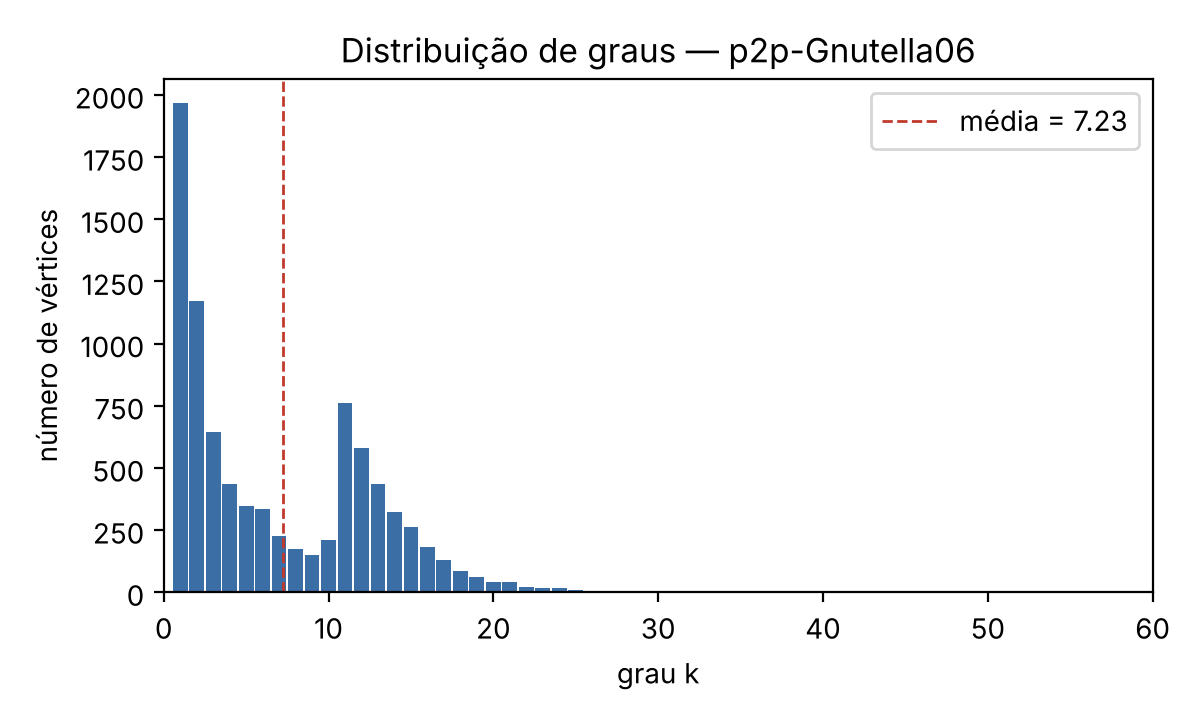
\includegraphics[width=\linewidth]{distribuicao_graus.png}
  \caption{Distribuição de graus. É bimodal, com um pico em $k=1$ e outro em
  $k\approx 11$, e a média (7,23) cai num vale entre os dois picos.}
  \Description{Histograma de graus com dois picos.}
  \label{fig:graus}
\end{figure}

\textbf{Comentários.} O grafo é muito esparso: a densidade é $8{,}3\times10^{-4}$,
ou seja, existem menos de 0,1\% das arestas possíveis. Mesmo assim, ele é conexo e
as distâncias são curtas (Figura~\ref{fig:dist}): 86,3\% dos pares estão a até 5
saltos e 99,97\% a até 7 saltos. A excentricidade varia de 6 (o centro tem 338
vértices) a 10 (a periferia tem só 4 vértices). A Figura~\ref{fig:graus} mostra que
a distribuição de graus \emph{não} é unimodal. Investigamos o motivo na
Seção~\ref{sec:descoberta}. A clusterização é muito baixa: há só 1.142 triângulos,
e 85,5\% dos vértices não participam de nenhum. A visualização
(Figura~\ref{fig:vis}) mostra hubs de grau alto ligados a muitos vértices de grau
baixo, e poucos ciclos curtos entre esses vértices.

\begin{figure}[t]
  \centering
  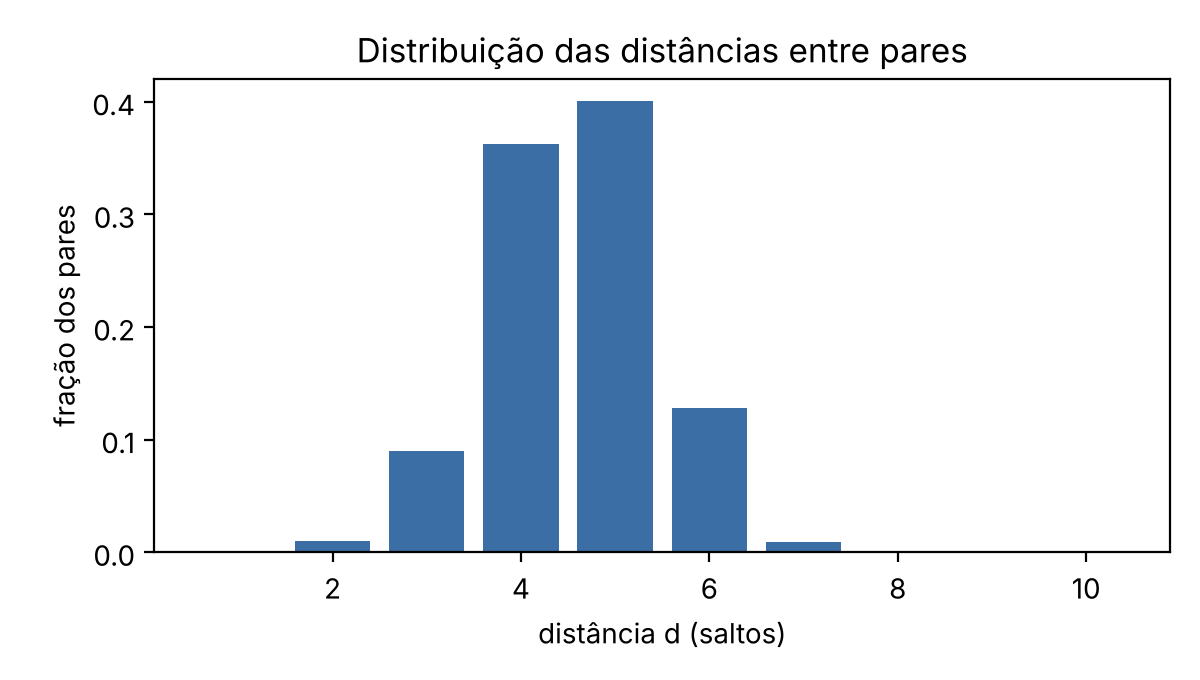
\includegraphics[width=0.92\linewidth]{distribuicao_distancias.png}
  \caption{Distribuição das distâncias entre todos os pares de vértices. A moda é 5
  e a média é 4,57.}
  \Description{Histograma das distâncias, concentrado entre 3 e 6.}
  \label{fig:dist}
\end{figure}

\begin{figure}[t]
  \centering
  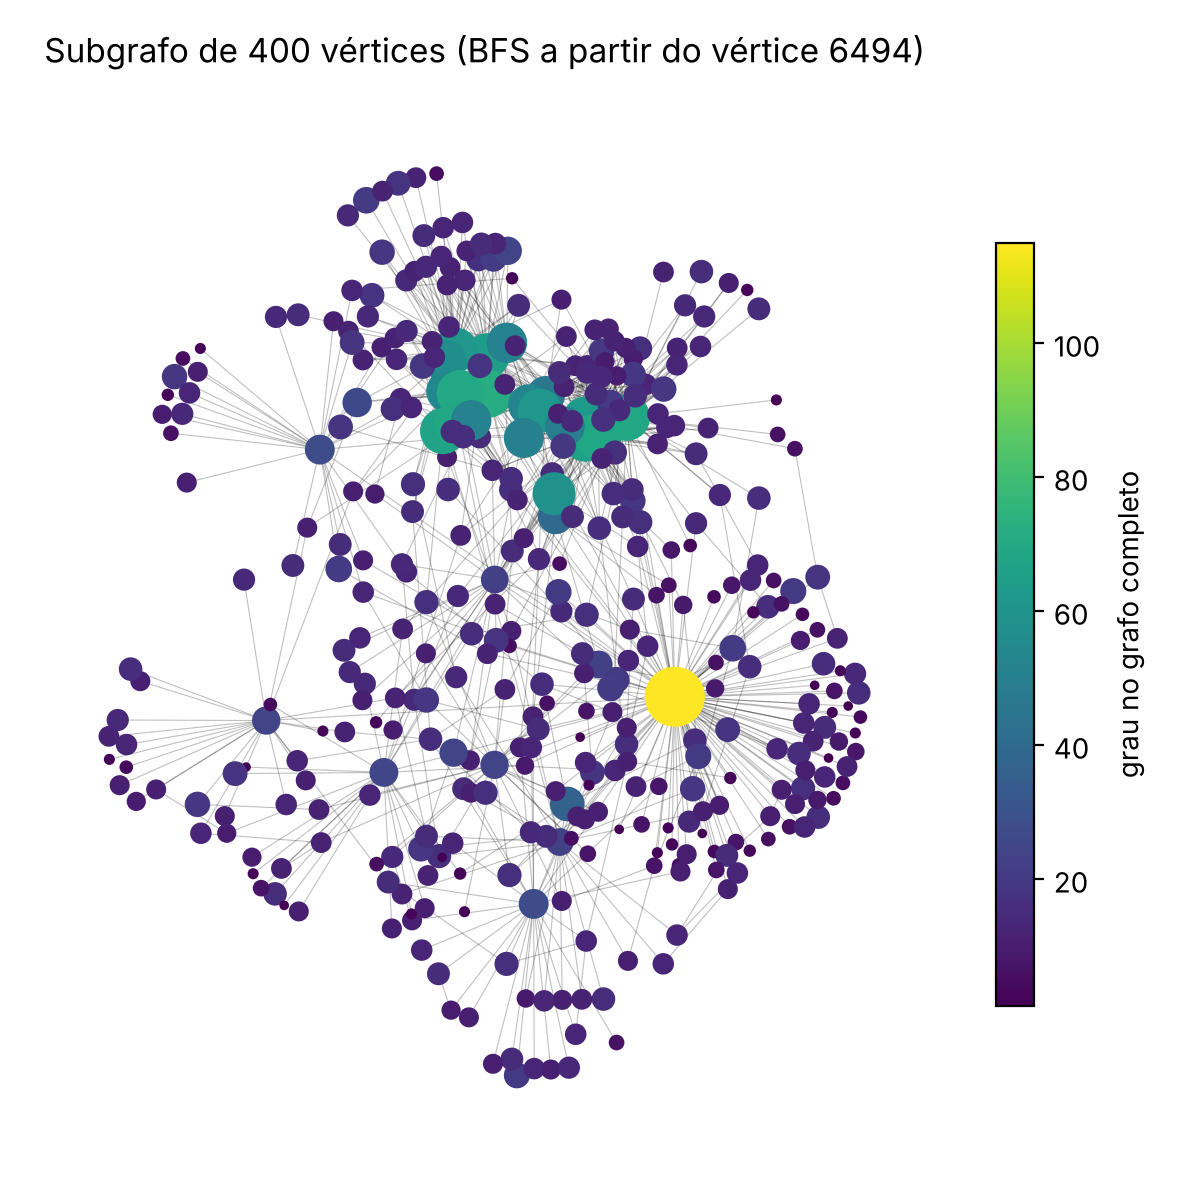
\includegraphics[width=0.85\linewidth]{visualizacao_subgrafo.png}
  \caption{Visualização reduzida: subgrafo induzido pelos 400 primeiros vértices de
  um BFS a partir do vértice de maior grau (6494, grau 115). O tamanho e a cor
  indicam o grau no grafo completo.}
  \Description{Desenho de rede com um grande hub amarelo e vários hubs médios.}
  \label{fig:vis}
\end{figure}

\subsection{Parte II --- Algoritmos da disciplina}\label{sec:p2}
\textbf{Corretude.} Os resultados de todos os algoritmos são consistentes entre si:
\begin{itemize}
  \item o BFS e o DFS a partir do vértice 0 alcançam os 8.717 vértices (o grafo é conexo);
  \item Dijkstra e Bellman-Ford devolvem exatamente as distâncias do BFS;
  \item o Floyd-Warshall vetorizado é idêntico à versão com três laços em Python
  puro (subgrafo de 150 vértices). No grafo inteiro, ele confirmou diâmetro 10,
  raio 6 e $L=4{,}572$;
  \item Prim e Kruskal produzem árvores geradoras com 8.716 arestas e peso 8.716
  ($=|V|-1$, já que os pesos são unitários);
  \item as componentes fortemente conexas do Tarjan coincidem com as do NetworkX.
\end{itemize}

O grafo \textbf{não é euleriano}: é conexo, mas 5.088 vértices têm grau ímpar, então
não admite nem circuito nem caminho euleriano (seriam necessários 0 ou 2 vértices
de grau ímpar). No grafo dirigido, o Tarjan encontrou 5.492 componentes fortemente
conexas. A maior tem 3.226 vértices (37,0\%) e as outras 5.491 são unitárias.

\textbf{Tempo real e complexidade.} A Tabela~\ref{tab:tempos} compara a
complexidade teórica, o tempo real (30 execuções, IC de 95\% pela Normal) e o
expoente $b$ observado. A Figura~\ref{fig:escala} mostra o crescimento em escala
log-log.

\begin{table*}[t]
\caption{Complexidade teórica e tempo real no grafo completo ($|V|=8.717$,
$|E|=31.525$; $n=30$ execuções; IC de 95\% com $z=1{,}96$). $b$ é o expoente do
ajuste $t\propto (V+E)^b$ nos subgrafos crescentes; para o Floyd-Warshall,
$t\propto V^b$.}
\label{tab:tempos}
\begin{tabular}{@{}llrrrr@{}}
\toprule
Algoritmo & Compl. teórica & Média (ms) & Desvio (ms) & IC 95\% (ms) & $b$ obs. \\
\midrule
BFS & $O(V+E)$ & 5,74 & 1,31 & [5,27; 6,21] & 0,91 \\
DFS (iterativa) & $O(V+E)$ & 13,62 & 3,84 & [12,25; 15,00] & 0,84 \\
Verificação de eulerianidade & $O(V+E)$ & 7,20 & 1,78 & [6,56; 7,84] & 0,83 \\
Dijkstra (heap binário) & $O((V+E)\log V)$ & 12,46 & 0,70 & [12,21; 12,71] & 0,91 \\
Bellman-Ford (parada antecipada) & $O(V\cdot E)$ & 53,16 & 15,63 & [47,57; 58,75] & 1,00 \\
Tarjan (CFC, grafo dirigido) & $O(V+E)$ & 12,67 & 7,70 & [9,92; 15,42] & 0,84 \\
Kruskal (union-find) & $O(E\log E)$ & 23,10 & 0,74 & [22,83; 23,36] & 0,97 \\
Prim (heap binário) & $O(E\log V)$ & 35,63 & 6,43 & [33,33; 37,93] & 1,14 \\
Floyd-Warshall ($V=1000$, $E=2456$) & $\Theta(V^3)$ & 1.130,88 & 45,08 & [1.114,75; 1.147,02] & 3,08 \\
Floyd-Warshall (grafo completo, 1×) & $\Theta(V^3)$ & \multicolumn{3}{c}{1.040,8 s} & --- \\
\bottomrule
\end{tabular}
\end{table*}

\begin{figure}[t]
  \centering
  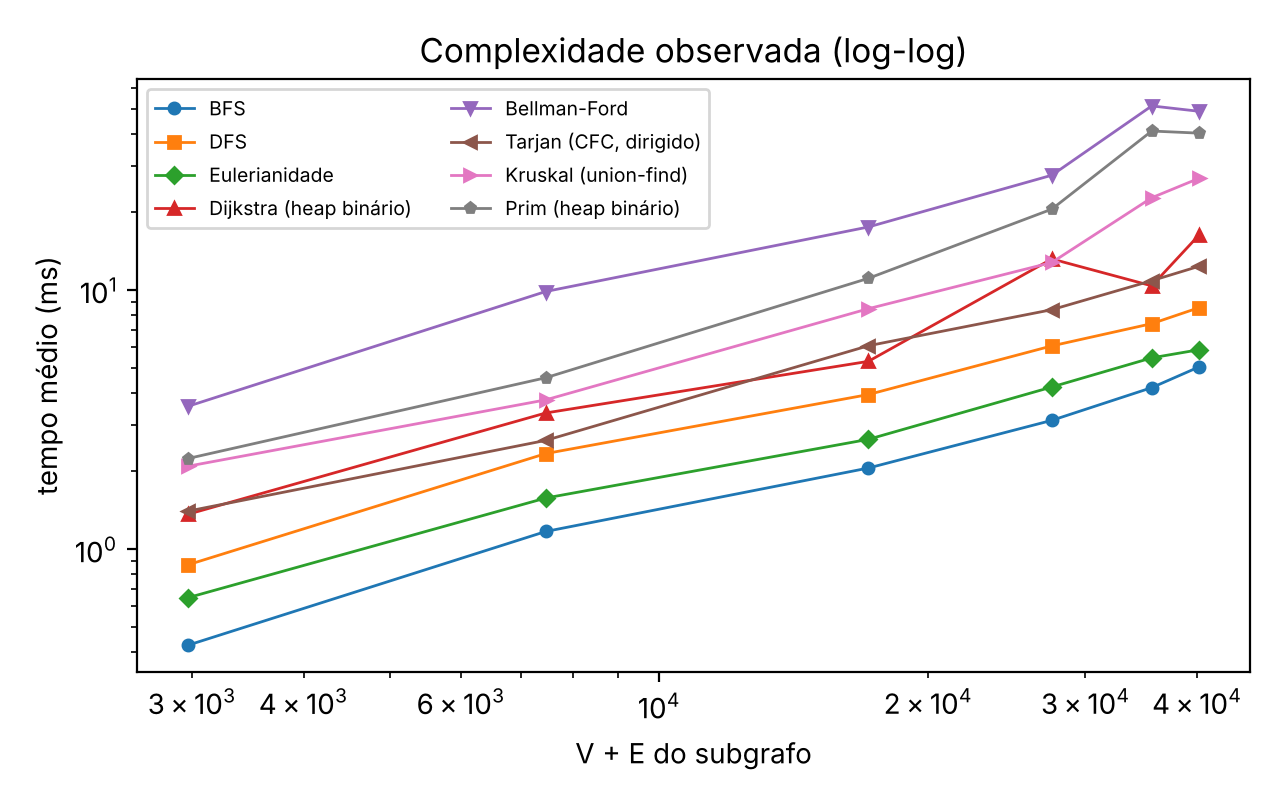
\includegraphics[width=\linewidth]{escalabilidade_algoritmos.png}
  \caption{Tempo médio (10 execuções por ponto) em função de $V+E$ para subgrafos
  crescentes, em escala log-log. Inclinação próxima de 1 indica crescimento linear.}
  \Description{Oito retas aproximadamente paralelas em escala log-log.}
  \label{fig:escala}
\end{figure}

\begin{figure}[t]
  \centering
  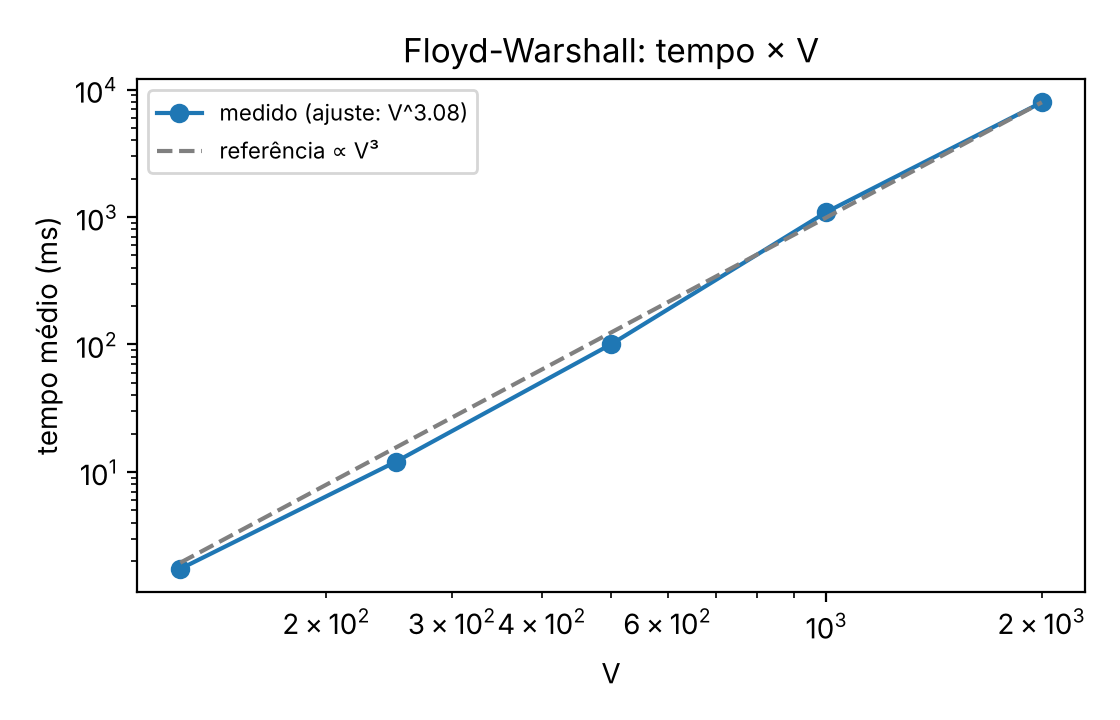
\includegraphics[width=0.9\linewidth]{escalabilidade_floyd_warshall.png}
  \caption{Floyd-Warshall: tempo em função de $V$ (125 a 2.000 vértices). O ajuste
  dá expoente 3,08, praticamente igual à referência $V^3$.}
  \Description{Pontos medidos acompanhando a reta de referência V ao cubo.}
  \label{fig:fw}
\end{figure}

\textbf{Comentários.} Os algoritmos lineares (BFS, DFS, eulerianidade e Tarjan)
têm expoentes entre 0,83 e 0,91. Isso é compatível com $O(V+E)$: valores um pouco
abaixo de 1 aparecem porque o custo fixo do interpretador pesa mais nos subgrafos
pequenos. O DFS é cerca de 2,4 vezes mais lento que o BFS, embora tenha a mesma
complexidade. A versão iterativa empilha um vértice várias vezes e só o descarta
quando ele é desempilhado, o que muda a constante, não a ordem de crescimento.

Dijkstra, Prim e Kruskal ganham o fator logarítmico do heap ou da ordenação. Prim é
o mais custoso desse grupo ($b=1{,}14$) porque insere no heap uma entrada por
aresta. No Bellman-Ford, o limite $O(V\cdot E)$ supõe até $V-1=8.716$ rodadas, mas
com a parada antecipada (encerrar quando uma rodada não altera nenhuma distância)
bastaram 4 rodadas. Como a relaxação é feita no próprio vetor de distâncias, uma
rodada pode avançar vários níveis. O custo real fica $O(k\cdot E)$ com $k$ pequeno,
o que explica o expoente $b=1{,}00$ em $V+E$. Mesmo assim, ele é o mais lento dos
algoritmos lineares na prática, porque percorre todos os arcos a cada rodada.

O Floyd-Warshall confirma $\Theta(V^3)$ com $b=3{,}08$
(Figura~\ref{fig:fw}). No grafo completo, uma única execução levou 17,3~min,
enquanto um BFS levou 5,7~ms. Por isso as 30 repetições do Floyd-Warshall foram
feitas num subgrafo conexo de 1.000 vértices. Para obter todas as distâncias num
grafo esparso, $V$ execuções de BFS custam $O(V(V+E))$, contra $\Theta(V^3)$ do
Floyd-Warshall. Os desvios maiores (DFS, Bellman-Ford, Tarjan) vêm de variações do
coletor de lixo do Python e da carga da máquina. Mesmo nesses casos, os ICs são
estreitos (meia-largura menor que 25\% da média).

\subsection{Parte III --- Análise estrutural}

\subsubsection*{(1) Small-world}
Seguindo o Apêndice~A, calculamos $L$ e $C$ do grafo com código próprio e os
comparamos com 10 grafos aleatórios de Erdős--Rényi $G(n,m)$~\cite{erdos1959},
também gerados com código próprio, com o mesmo $n$ e o mesmo $m$ (e, portanto, o
mesmo grau médio). Em média, a maior componente do grafo aleatório cobre 99,9\% dos
vértices, e nela calculamos $L_{rand}$. A Tabela~\ref{tab:sw} mostra os resultados.

\begin{table}[t]
\caption{Small-world: grafo real × grafos aleatórios $G(n,m)$ equivalentes (média
± desvio de 10 instâncias) e valores teóricos de ER.}
\label{tab:sw}
\begin{tabular}{lrrr}
\toprule
 & Gnutella06 & $G(n,m)$ & Teórico ER \\
\midrule
$L$ & 4,572 & $4{,}808 \pm 0{,}002$ & $\ln n/\ln\langle k\rangle = 4{,}585$ \\
$C$ & 0,00668 & $0{,}00081 \pm 0{,}00014$ & $\langle k\rangle/n = 0{,}00083$ \\
\midrule
\multicolumn{4}{l}{$L/L_{rand} = 0{,}95$ \quad $C/C_{rand} = 8{,}2$ \quad
$\sigma = \frac{C/C_{rand}}{L/L_{rand}} = 8{,}6$} \\
\bottomrule
\end{tabular}
\end{table}

\textbf{Resposta.} Sim, \emph{há indícios} de mundo pequeno: $L \approx L_{rand}$
(o real é até 5\% menor) e $C$ é 8,2 vezes maior que $C_{rand}$, o que dá
$\sigma = 8{,}6 > 1$~\cite{watts1998}. A propriedade, porém, é \emph{fraca}. O
coeficiente absoluto ($0{,}0067$) é muito baixo quando comparado a redes sociais
típicas ($C \sim 0{,}1$--$0{,}6$), e a maior parte da razão $C/C_{rand}$ vem de os
dois valores serem minúsculos. Isso faz sentido para o Gnutella: os peers se
conectam a outros que descobrem pela rede, não a ``amigos em comum'', então quase não
se formam triângulos. Já os caminhos curtos são necessários. A implicação prática
é direta: no Gnutella, as buscas são inundações limitadas por TTL (tipicamente 7
saltos~\cite{ripeanu2002}), e, como 99,97\% dos pares estão a até 7 saltos, uma
consulta pode, em princípio, alcançar quase toda a rede. O custo disso é o tráfego
alto: com $C$ baixo, há pouca redundância local, e a inundação se espalha
rapidamente para muitos vértices diferentes.

\subsubsection*{(2) Lei de potência}
Seguindo o Apêndice~B, plotamos $P(k)$ e a CCDF em escala log-log
(Figura~\ref{fig:pl}). Ajustamos uma reta por mínimos quadrados e também o
estimador de máxima verossimilhança discreto de Clauset et al.~\cite{clauset2009},
com $k_{min}$ escolhido pela menor distância de Kolmogorov--Smirnov.

\begin{figure*}[t]
  \centering
  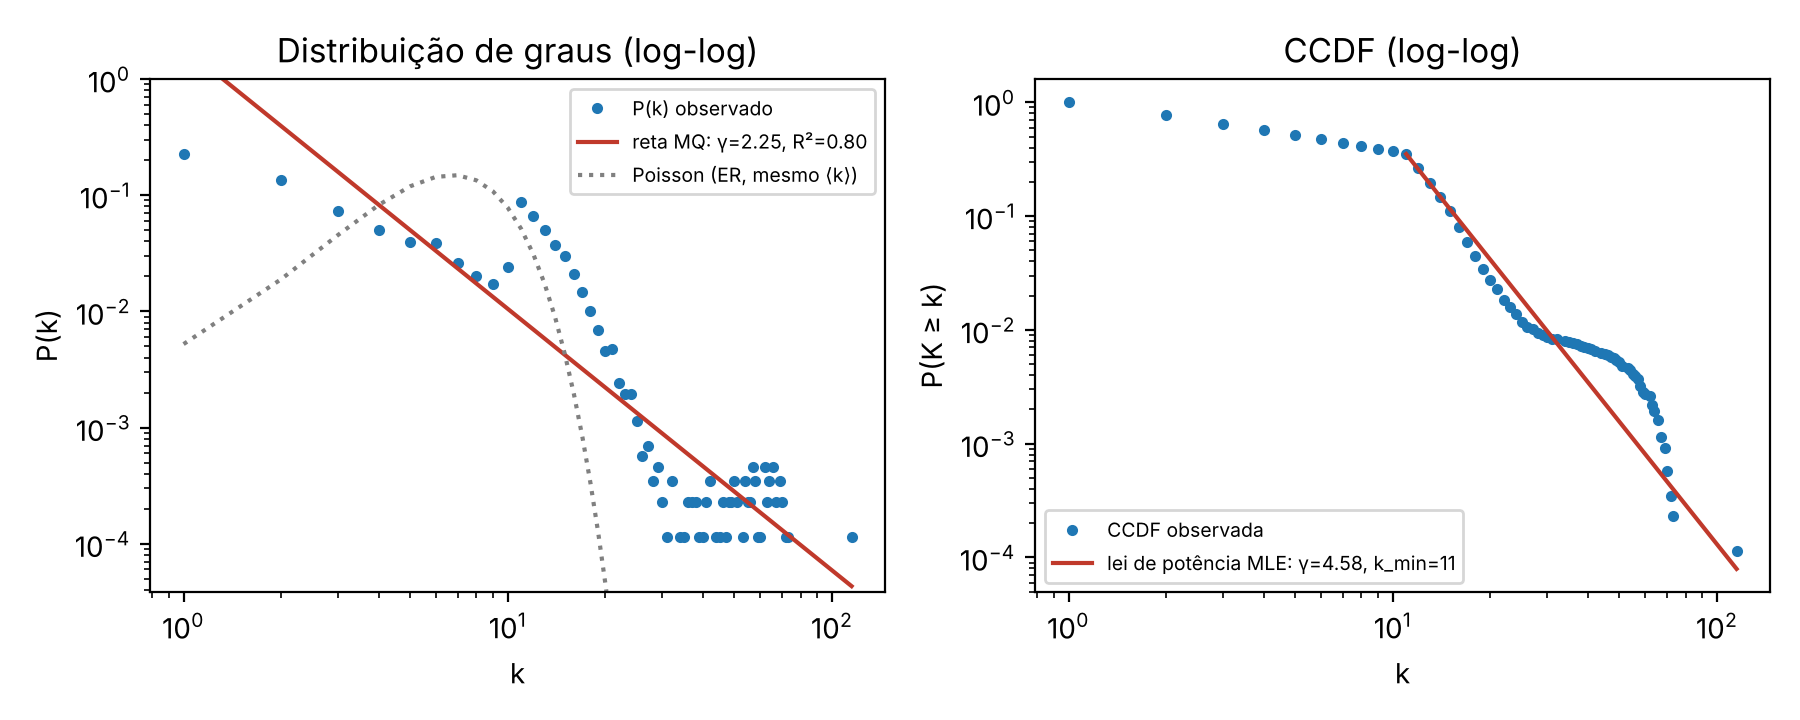
\includegraphics[width=0.85\linewidth]{lei_de_potencia.png}
  \caption{Esquerda: $P(k)$ em log-log com a reta de mínimos quadrados e a Poisson
  de um grafo ER com o mesmo $\langle k\rangle$. Direita: CCDF com a lei de potência
  ajustada por máxima verossimilhança para $k \ge 11$.}
  \Description{Distribuição de graus em log-log com uma corcova em k≈11, que não
  forma uma reta.}
  \label{fig:pl}
\end{figure*}

\textbf{Resposta.} \emph{Não}. Para haver lei de potência, $\log P(k)$ precisaria ser
aproximadamente linear em $\log k$, e não é. A reta de mínimos quadrados explica só
$R^2 = 0{,}80$ de $P(k)$ ($\gamma \approx 2{,}25$), e a curva tem uma corcova
evidente em $k\approx 11$ (Figura~\ref{fig:pl}), que reflete a bimodalidade da
Figura~\ref{fig:graus}. Na cauda ($k\ge 11$), a máxima verossimilhança dá
$\gamma = 4{,}58$, bem acima da faixa $2<\gamma<3$ típica de redes livres de
escala~\cite{barabasi1999}. Além disso, a CCDF tem um platô entre $k\approx 30$ e
$70$ seguido de queda abrupta, e o grau máximo é só 115 ($\approx 16\langle
k\rangle$). A distribuição é mais dispersa que uma Poisson (coeficiente de variação
$\approx 1$, contra $1/\sqrt{\langle k\rangle} \approx 0{,}37$ para ER), mas a
cauda é limitada: não há hubs extremos. Esse resultado está de acordo com
Ripeanu et al.~\cite{ripeanu2002}, que já em 2001 observaram que a distribuição de
graus do Gnutella não seguia uma lei de potência pura.

\subsubsection*{(3) Robustez}
Seguindo o Apêndice~C, trabalhamos na maior componente (o grafo inteiro),
com $n=8.717$ e $r=\lceil 0{,}05n\rceil = 436$. Na remoção aleatória, fizemos
$T=30$ repetições. No ataque direcionado, usamos a centralidade de \textbf{grau}
com ranking fixo: removemos os 436 vértices de maior grau (todos com grau $\ge 17$),
o que elimina 32,1\% das arestas. Os resultados estão na Tabela~\ref{tab:rob} e na
Figura~\ref{fig:rob}.

\begin{table*}[t]
\caption{Robustez à remoção de 5\% dos vértices ($r=436$). Aleatória: média ±
desvio e IC de 95\% ($T=30$, Normal). Direcionada: remoção dos 5\% de maior grau.}
\label{tab:rob}
\begin{tabular}{lrrrr}
\toprule
Métrica & Original & Aleatória (média ± dp) & IC 95\% & Direcionada (grau) \\
\midrule
A: $S$ = tamanho da maior componente / $n$ & 1,000 & $0{,}938 \pm 0{,}002$ & [0,938; 0,939] & 0,912 \\
A': maior componente / vértices restantes & 1,000 & $0{,}988 \pm 0{,}002$ & [0,987; 0,988] & 0,960 \\
B: número de componentes $c$ & 1 & $100{,}9 \pm 15{,}0$ & [95,5; 106,3] & 330 \\
C: distância média na maior componente & 4,572 & $4{,}617 \pm 0{,}008$ & [4,614; 4,620] & 5,173 \\
C': diâmetro da maior componente & 10 & $9{,}7 \pm 0{,}5$ & [9,5; 9,9] & 11 \\
D: fração de vértices isolados & 0 & $0{,}0119 \pm 0{,}0018$ & [0,0112; 0,0125] & 0,0397 \\
\bottomrule
\end{tabular}
\end{table*}

\begin{figure*}[t]
  \centering
  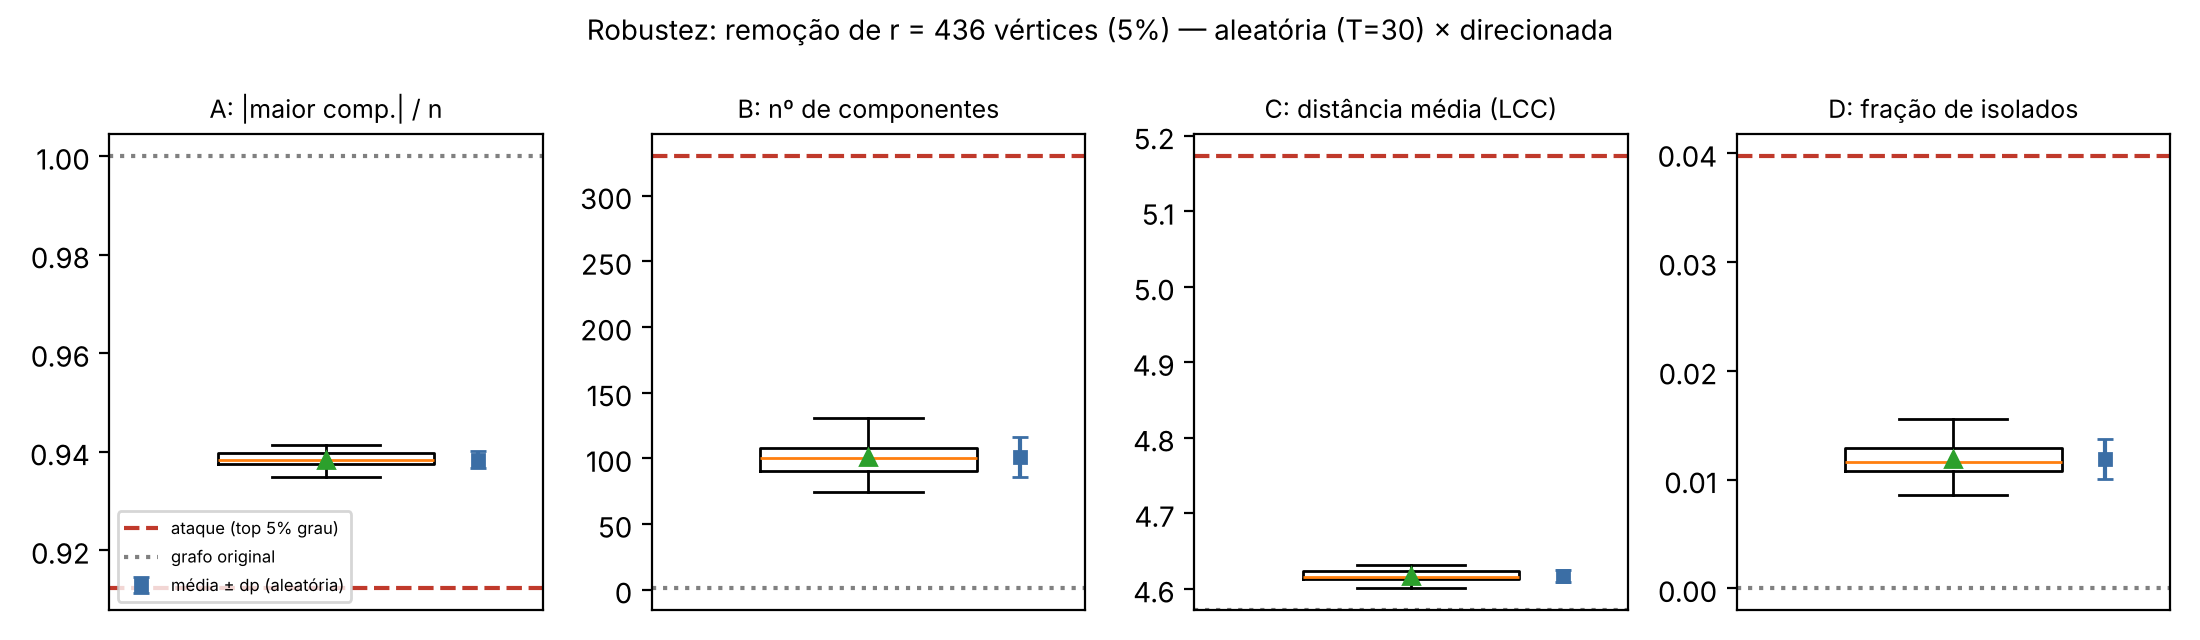
\includegraphics[width=0.95\linewidth]{robustez_boxplot.png}
  \caption{Boxplots das 30 remoções aleatórias, com a média ± desvio padrão
  (quadrado azul). A linha vermelha tracejada é o ataque direcionado e a pontilhada
  cinza é o grafo original.}
  \Description{Quatro boxplots; em todos o ataque fica bem fora da faixa da remoção aleatória.}
  \label{fig:rob}
\end{figure*}

\textbf{Resposta (a): sim, a rede é robusta à remoção aleatória.} A maior componente
mantém 98,8\% dos vértices restantes. As cerca de 100 componentes extras são quase
todas vértices isolados (1,2\%, isto é, folhas de grau 1 cujo único vizinho foi
removido). A distância média aumenta só 1\% e o diâmetro chega a diminuir.

\textbf{Resposta (b): a rede é mais sensível ao ataque direcionado, mas não colapsa
com 5\%.} Comparado à remoção aleatória, o ataque gera 3,3 vezes mais componentes
($c_{cent}=330 \gg c_{rand}=101$), 3,3 vezes mais vértices isolados e aumenta a
distância média em 12\% (de 4,62 para 5,17), com diâmetro 11. Em todas as métricas,
o ataque fica muito fora do IC da remoção aleatória. Ainda assim,
$S_{rand}=0{,}938$ e $S_{cent}=0{,}912$ são próximos, ou seja, não vale
$S_{rand} \gg S_{cent}$. Segundo o critério do Apêndice~C, a rede é
\emph{moderadamente} vulnerável a ataques. Ela não tem o colapso abrupto de redes
livres de escala~\cite{albert2000}, porque seus vértices mais centrais não
concentram tanto as conexões (o grau máximo é 115). Isso é coerente com a resposta
negativa sobre lei de potência.

\subsubsection*{(4) Descoberta mais interessante}\label{sec:descoberta}
Para entender a distribuição bimodal, separamos os vértices pelo \emph{grau de
saída} no arquivo dirigido original (Figura~\ref{fig:desc}).
\begin{itemize}
  \item \textbf{4.978 vértices (57,1\%) têm grau de saída 0.} São peers que aparecem
  apenas como vizinhos de outros, ou seja, foram descobertos, mas nunca rastreados
  pelo \textit{crawler}. Eles têm grau mediano 2 (média 3,3) e formam o pico em $k=1$--$2$.
  \item \textbf{Não existe nenhuma aresta entre dois vértices não rastreados.} Isso
  confirma a hipótese: uma aresta só é registrada quando ao menos uma das pontas foi
  rastreada.
  \item Os 3.739 vértices rastreados têm grau mediano 12, e \textbf{66\% deles têm
  grau de saída exatamente 10}. Isso sugere um limite padrão de conexões do cliente
  Gnutella (ou da coleta) e explica o segundo pico em $k\approx 11$.
  \item Os 75 vértices de grau $\ge 30$, responsáveis pelo platô da CCDF, têm em
  média 38 arestas \emph{de entrada}: são peers populares, citados por muitos
  outros. Provavelmente eram \textit{ultrapeers}.
\end{itemize}
Essa estrutura de ``núcleo rastreado + folhas'' explica, ao mesmo tempo, quatro
resultados anteriores: (i) a bimodalidade dos graus e a ausência de lei de
potência; (ii) a clusterização baixa, porque folhas não rastreadas nunca fecham
triângulos entre si; (iii) os 5.491 componentes fortemente conexos unitários do
Tarjan, já que 4.978 deles são vértices sem arco de saída, que não podem estar em
nenhum ciclo dirigido; e (iv) os vértices isolados que surgem na análise de
robustez. A lição é que \textbf{parte do que se mede no grafo é propriedade do
processo de coleta, e não da rede P2P}.

\begin{figure*}[t]
  \centering
  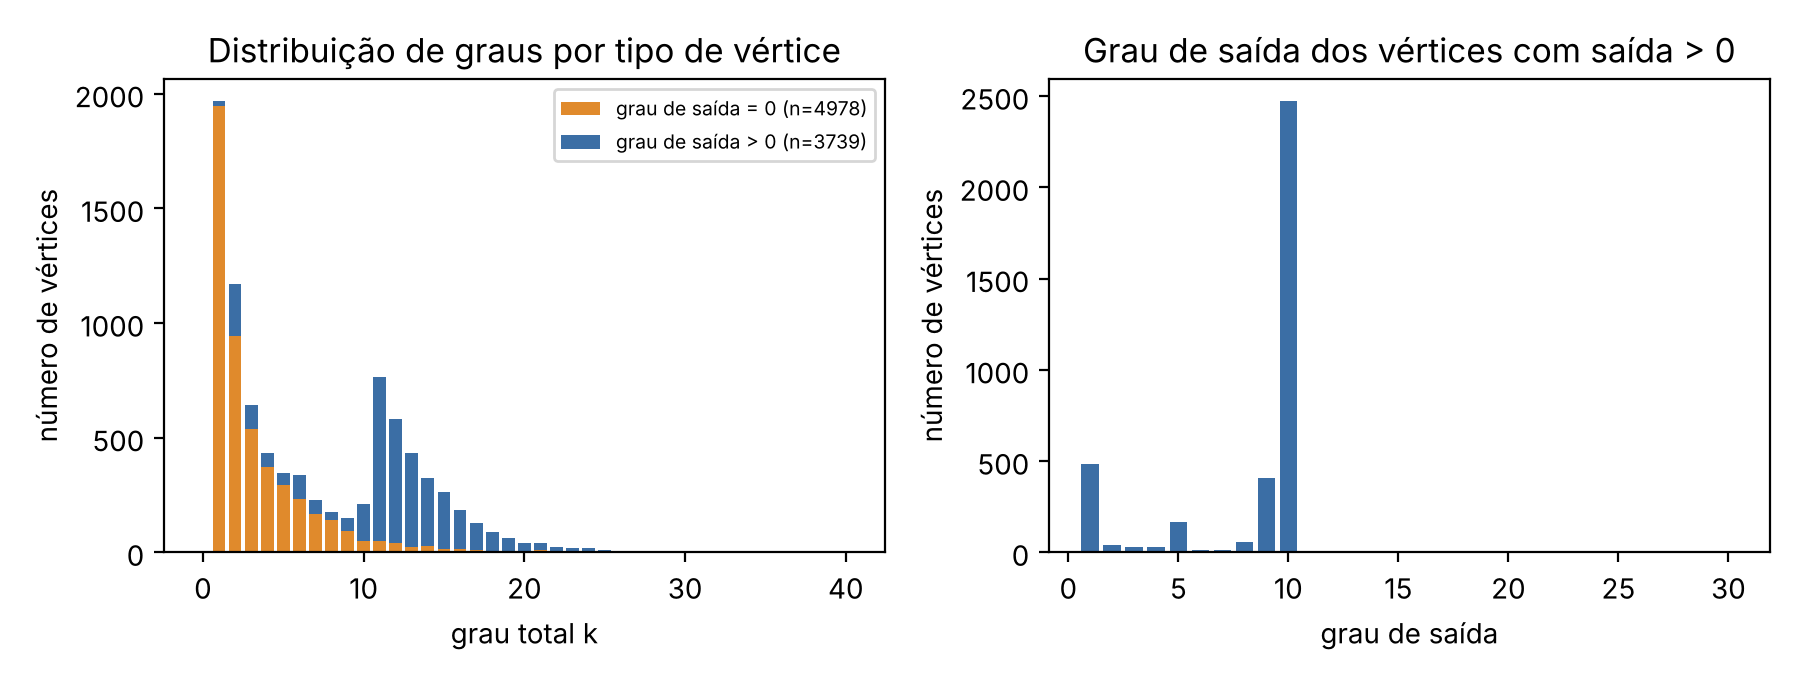
\includegraphics[width=0.85\linewidth]{descoberta_crawler.png}
  \caption{Esquerda: a distribuição de graus é a soma de duas populações, os
  vértices não rastreados (laranja, grau de saída 0) e os rastreados (azul).
  Direita: grau de saída dos rastreados, concentrado em 10.}
  \Description{Histograma empilhado com o pico de grau baixo em laranja e o pico em 11 em azul.}
  \label{fig:desc}
\end{figure*}

\section{Discussão crítica}
\textbf{Escolhas de tratamento.} Converter o grafo para não direcionado é adequado
às conexões P2P e permitiu calcular diâmetro, raio e caminho médio num grafo
conexo. Por outro lado, isso esconde a assimetria que deu origem à principal
descoberta. Como o cabeçalho do SNAP indica que cada par é salvo uma única vez, a
direção dos arcos não deve ser lida como sentido de comunicação. Ela representa,
mais provavelmente, quem foi rastreado. Por isso, o resultado do Tarjan deve ser
lido com cautela.

\textbf{Limitações.} (i) Com pesos unitários, Dijkstra, Bellman-Ford e as árvores
geradoras mínimas são casos triviais (as distâncias coincidem com o BFS e qualquer
árvore geradora é mínima). Eles foram executados para medir a complexidade, mas não
revelam estrutura nova. (ii) Os tempos medidos em Python incluem o custo do
interpretador e variam com a carga da máquina. Os valores absolutos não se
transferem para outras linguagens, mas os expoentes sim. (iii) O Floyd-Warshall foi
vetorizado com NumPy, o que reduz a constante, mas não muda a complexidade
$\Theta(V^3)$, confirmada empiricamente. (iv) O critério de mundo pequeno depende do
modelo nulo: usamos $G(n,m)$, que preserva $n$ e $\langle k\rangle$ mas não a
sequência de graus, então parte da diferença em $C$ pode vir da heterogeneidade dos
graus. (v) No ataque, usamos apenas a centralidade de grau com ranking fixo.
Recalcular o ranking após cada remoção, ou usar \textit{betweenness}, tenderia a
causar dano maior. (vi) A análise é de um único instante (6/ago/2002) e de uma
amostra parcial da rede, limitada pelo crawler.

\section{Conclusão}
O \textit{p2p-Gnutella06} é um grafo esparso e conexo, com distâncias curtas
(diâmetro 10, $L=4{,}57$) e clusterização muito baixa. Ele mostra indícios fracos
de mundo pequeno ($\sigma=8{,}6$), e esses caminhos curtos são o que permite buscas
por inundação com TTL pequeno. A distribuição de graus não segue lei de potência:
ela é bimodal, com cauda limitada. A rede é robusta a falhas aleatórias e só
moderadamente vulnerável a ataques aos vértices de maior grau. Os nove algoritmos
implementados produziram resultados consistentes entre si e com bibliotecas de
referência, e seus tempos reais confirmaram as complexidades teóricas (expoentes
$\approx 1$ para os lineares e $3{,}08$ para o Floyd-Warshall). A descoberta
central é que a estrutura do grafo é moldada pelo processo de coleta: 57\% dos
vértices nunca foram rastreados e não se ligam entre si. Esse fato explica a
bimodalidade, a baixa clusterização e as componentes fortemente conexas unitárias.

\textbf{Repositório} (códigos, dados tratados e README de execução):\\ \repo.

\bibliographystyle{ACM-Reference-Format}
\bibliography{refs}

\end{document}
